\documentclass[conference]{IEEEtran}

\usepackage[T1]{fontenc}
\usepackage[utf8]{inputenc}
\usepackage{amsmath,amssymb}
\usepackage{graphicx}
\usepackage{booktabs}
\usepackage{cite}
\usepackage{url}
\usepackage{xcolor}
\usepackage{algorithm}
\usepackage{algpseudocode}

\graphicspath{{figures/}}

\author{
\IEEEauthorblockN{Gaurav Guddeti}
\IEEEauthorblockA{Dept. of Artificial Intelligence\\
Vishwakarma University\\
Pune, India\\
guddetigaurav1@gmail.com}
\and
\IEEEauthorblockN{Aishwarya Zinjurtee}
\IEEEauthorblockA{Dept. of Artificial Intelligence\\
Vishwakarma University\\
Pune, India\\
aishwaryazinjurte148@gmail.com}
\and
\IEEEauthorblockN{Sidesh Indalkar}
\IEEEauthorblockA{Dept. of Artificial Intelligence\\
Vishwakarma University\\
Pune, India\\
sideshindalkar@gmail.com}
}

\begin{document}

\title{SmartOPD: Occupant-Aware Computer Vision and Fuzzy Wait-Time Estimation for Outpatient Queue Management}

\maketitle

\begin{abstract}
Most small outpatient departments still run on paper tokens and a nurse calling
numbers out loud. Patients have no idea how long they will wait, so they drift
towards the reception desk, and the clinic keeps no record of how long a
consultation actually takes. We describe SmartOPD, a system that uses one
ordinary camera to keep a digital queue in step with what happens at the
doctor's door. People are found with YOLO11n and followed by a small centroid
tracker, both running on the CPU of the same machine that serves the web
pages. Detections become occupants of the doctor-room zone. An entry counts
only after the person has stayed inside for a couple of seconds, people who are
already inside when tracking begins are treated as ghosts without a token, and
each exit is matched to the person who actually left, so a patient walking out
while another walks in does not disturb the queue. Consultation lengths are
kept as raw video seconds; an operator-set factor converts them to clinic
minutes, and a compact Mamdani fuzzy system combines the learned length, the
evidence behind it, the spread of past measurements, the queue position and the
progress of the ongoing consultation into a wait range with a confidence label.
Three browser screens share one FastAPI state store: a monitoring console, a
nurse desk and a patient display. The code is covered by 58 unit tests, and a
headless replay of a frame-continuous ping-pong clip completes six tokens in
order, with no token ever moving backwards and every consultation feeding the
estimator.
\end{abstract}

\begin{IEEEkeywords}
computer vision, person detection, multi-object tracking, outpatient
department, queue management, fuzzy logic, wait-time prediction, edge
inference
\end{IEEEkeywords}

\section{Introduction}

Walk into any busy outpatient department (OPD) and the same picture repeats:
people holding paper slips, a crowded corridor, and a nurse reading out token
numbers between other duties. The queue is real, but it is invisible to the
patient. Someone who arrived an hour ago has no way of knowing whether two or
ten people are still ahead of them. Blocking the queue on a single shared
display is therefore less a technical question than a communication problem.

The operations research community has studied outpatient scheduling for
decades. Reviews by Cayirli and Veral \cite{cayirli2003} and by Gupta and Denton
\cite{gupta2008} discuss appointment rules, panel sizes and overbooking, and
the queueing formulas behind the usual wait estimates are standard
\cite{gross2018}. Almost all of this work assumes that service times are known
from historical records, or that a clerk measures them. In a small clinic
neither is true. Nobody times the doctor, and the tokens are written on paper.

Cameras are already mounted in most such clinics, and a camera plus a modern
detector is enough to observe a waiting hall without touching any existing
process \cite{redmon2016yolo,redmon2018yolov3,ultralytics2024}. The difficulty
is not finding people in a frame. It is deciding what their movement means for
a queue: who has entered the room, who is only passing the open door, and which
token should be closed when somebody walks out.

This paper reports what we built and what we learned while answering those
questions. The contributions are as follows. First, an occupant-based room
model in which a token is attached to a tracked person only after a dwell
confirmed entry; people already inside are kept as token-less ghosts, and exits
are completed per occupant so that simultaneous entry and exit at the door
cannot corrupt the queue. Second, handling of looped video for demonstrations:
a ping-pong source lets tracker identities and consultations survive the wrap,
while jump-cut sources freeze events briefly and re-bind occupants afterwards.
Third, a fuzzy wait-time estimator that replaces the usual remainder plus
people-ahead-times-average formula with a Mamdani system over five linguistic
inputs, giving a range, a confidence tag and a phrase a patient can read.
Fourth, a reproducible implementation with three shared-state web interfaces,
58 unit tests and a replay harness that checks ordering and no-backwards
invariants on a real clip.

The rest of the paper follows the system. Section~\ref{sec:related} reviews
related work, Section~\ref{sec:arch} describes the architecture,
Sections~\ref{sec:vision} and~\ref{sec:queue} cover the vision pipeline and the
queue rules, Section~\ref{sec:fuzzy} presents the estimator and
Section~\ref{sec:ui} the interfaces. Section~\ref{sec:eval} reports the
evaluation, Section~\ref{sec:limits} the limitations, and
Section~\ref{sec:concl} concludes.

\section{Related Work}
\label{sec:related}

\subsection{Person detection and tracking}
Single-stage detectors such as YOLO regress boxes and class scores in one pass
and have become the default choice for real-time person detection
\cite{redmon2016yolo,redmon2018yolov3}. The YOLO11 family offers small weights
that run acceptably on a CPU \cite{ultralytics2024}, which matters when the
camera is attached to a clinic computer rather than a GPU server. Tracking is
almost always built on detection: SORT \cite{bewley2016sort} associates boxes
with a Kalman filter and Hungarian assignment, DeepSORT
\cite{wojke2017deepsort} adds an appearance embedding, and ByteTrack
\cite{zhang2022bytetrack} also uses low-confidence boxes. For a fixed camera
looking at one room, we found that greedy nearest-neighbour association on the
foot point is enough, at the price of identity switches when someone is hidden
for several seconds.

\subsection{Crowd analytics}
Crowd counting and density estimation from images is a mature field, surveyed
by Sindagi and Patel \cite{sindagi2018}. Reported results are mostly head-count
errors on public benchmarks. A queue needs something different: discrete door
events, tied to individual people, that survive occlusion and can be attributed
to named tokens.

\subsection{Outpatient scheduling and queueing}
The appointment scheduling literature \cite{cayirli2003,gupta2008} optimises
interval lengths and overbooking given a service-time distribution, and
classical queueing theory \cite{gross2018} provides the standard wait
expressions. Our crisp baseline is essentially the pollaczek-khinchine style
average with a measured mean; the fuzzy layer replaces it once the mean becomes
uncertain. What is missing in this literature, and what a camera can supply, is
the measurement itself.

\subsection{Fuzzy decision support}
Fuzzy sets \cite{zadeh1965fuzzy} and Mamdani inference \cite{mamdani1975} are
still useful when inputs are imprecise and the rules must be explainable
\cite{ross2010fuzzy}. Telling a patient that the wait is ``about ten minutes,
medium confidence'' is more honest than printing a single number that pretends
to be exact.

\section{System Architecture}
\label{sec:arch}

Figure~\ref{fig:arch} shows the arrangement. One Python process serves both the
vision pipeline and the web application. A background thread reads frames, runs
detection and tracking, and updates the queue engine; FastAPI
\cite{fastapi2024} exposes a JSON API and three pages. The queue state is
written to a local JSON file every two seconds with an atomic replace, so an
abrupt shutdown leaves either the previous or the new file, never half of one.
Frames stay in memory. Only anonymous counters, token numbers, durations and
zone rectangles are stored. After installation the system does not contact any
external service.

\begin{figure*}[t]
\centering
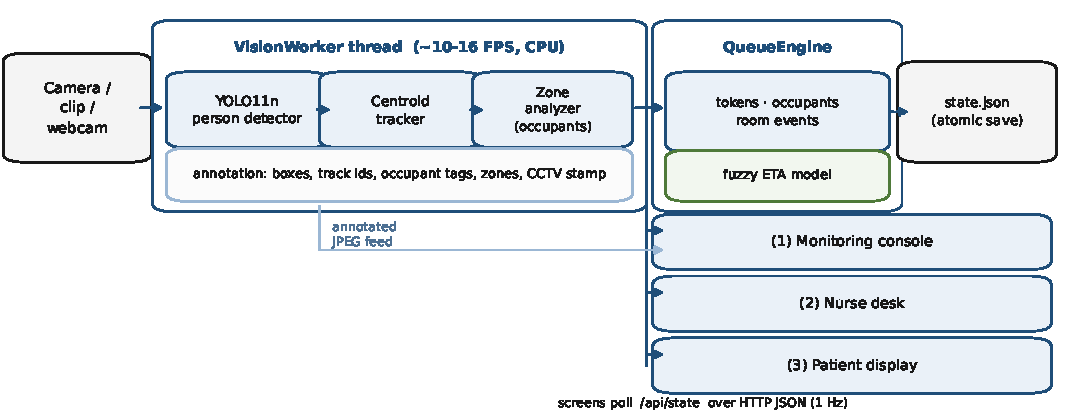
\includegraphics[width=\textwidth]{fig_architecture.pdf}
\caption{System architecture. The vision worker runs YOLO11n, a centroid
tracker and the zone analyzer; the queue engine holds tokens, occupants and the
fuzzy estimator. The annotated JPEG stream feeds the monitoring console, and
all three screens poll \texttt{/api/state}.}
\label{fig:arch}
\end{figure*}

\begin{table}[t]
\caption{Interfaces and their users}
\label{tab:ui}
\centering
\small
\begin{tabular}{@{}p{1.3cm}p{1.3cm}p{3.9cm}@{}}
\toprule
Interface & User & Function \\
\midrule
Monitoring console & operator & annotated feed, zone drawing,
crowd counters, reason-coded event log \\
Nurse desk & nurse & registration, token issue, call, skip, no-show, undo,
time-factor slider, CSV export \\
Patient display & patients & now-serving board, next-up token, per-token
wait range with confidence \\
\bottomrule
\end{tabular}
\end{table}

\section{Vision Pipeline}
\label{sec:vision}

\subsection{Detection}
Each processed frame is resized to 640\,px and passed to YOLO11n restricted to
the \texttt{person} class at a confidence threshold of 0.35
\cite{ultralytics2024}. On the laptop CPU we used for development the pipeline
settles between 10 and 16 processed frames per second. That is well below the
camera rate, and deliberately so: a queue changes on the scale of seconds, and
processing every frame would only waste CPU.

\subsection{Tracking}
Detections are attached to existing tracks by greedy nearest-neighbour matching
on the foot point $(c_x,c_y)$ of each box,
\begin{equation}
\hat{j} = \operatorname*{arg\,min}_{j:\ \lVert c_i-d_j\rVert_2 < d_{\max}}
\lVert c_i-d_j\rVert_2 ,
\end{equation}
with $d_{\max}=0.18$ in normalized coordinates. A track survives 15 consecutive
misses, roughly 1.5\,s at our frame rate, before it expires. Expiry is reported
to the analyzer as a possible door event rather than silently dropped.

\subsection{Occupants, ghosts and exits}
\label{sec:occupants}
A token is a human artifact and a track is a machine artifact; the analyzer
exists to keep the two from being confused. It maintains a set of occupants
$\mathcal{O}=\{(k,\tau,t_{\mathrm{in}})\}$, where $k$ is a track key, $\tau$ the
linked token or $\varnothing$, and $t_{\mathrm{in}}$ the moment the person was
first seen inside the doctor zone. Three rules do most of the work.

An entry needs a sighting outside and a dwell. A track seen in the waiting area
that moves inside the doctor zone is confirmed only after
$\Delta_{\mathrm{entry}}=2$\,s of continuous presence,
\begin{equation}
\text{entry}(k) \iff t_{\mathrm{in}}\ \text{recorded}\ \wedge\
(t_{\mathrm{now}}-t_{\mathrm{in}}) \ge \Delta_{\mathrm{entry}} .
\end{equation}
Shorter crossings are written to the log as pass-bys and touch no token.
Someone who is inside at tracking start, or who appears inside without ever
being seen outside, becomes a ghost: an occupant with $\tau=\varnothing$ that
holds the room but cannot consume a token. This case is not hypothetical. In
our clip the woman is already in the cabin when the video begins, and without
the ghost rule her exit would have closed the first patient's consultation
before it started.

Exits are per occupant. An occupant leaves when the foot point stays outside
the zone for four consecutive frames (one dropped detection cannot end a
consultation) or when the track vanishes at the door. Only the leaver's token
is completed. In a swap, one patient walking out while the next walks in, the
two events are independent and the queue advances exactly once.

Tokens never move backwards. The camera may only take a token from
\texttt{waiting} to \texttt{called} to \texttt{in} to \texttt{done}. An earlier version
of this system reverted an admission when the measured stay looked too short.
On short demonstration clips that rule oscillated, and we removed it. Noise
protection now happens before admission, never after.

\subsection{Seams and continuous loops}
\label{sec:seam}
A demonstration clip lasts seconds while a consultation lasts minutes, and the
clip has to loop. Two mechanisms bridge the gap. For the demo we build a
ping-pong source by concatenating the clip with its reverse. Every join and the
wrap are frame-continuous, so the tracker is not reset and a consultation can
span several loops. Ordinary sources with a jump cut behave differently: the
seam freezes events for $\Delta_{\mathrm{hold}}=1.5$\,s, the tracker is reset,
and occupants are re-bound to whoever the camera sees afterwards
(Algorithm~\ref{alg:rebind}). Occupants without a visible track are kept, not
guessed away, because a wrong guess would close somebody's consultation.

\begin{algorithm}[t]
\caption{Seam re-binding of occupants}
\label{alg:rebind}
\begin{algorithmic}[1]
\State freeze entry and exit events for $\Delta_{\mathrm{hold}}$
\State reset the tracker; occupants survive, track keys do not
\State once the hold expires, take the set $I$ of keys inside the zone
\State order occupants: token-bearing first, then by $t_{\mathrm{in}}$
\For{$i \leftarrow 1$ \textbf{to} $\min(|I|,|\mathcal{O}|)$}
  \State re-key $\mathcal{O}_i$ to $I_i$ and clear its miss counter
\EndFor
\State every remaining key in $I$ becomes a new ghost occupant
\State occupants without a track are kept
\State log \textsc{rebound} with the three counts
\end{algorithmic}
\end{algorithm}

\subsection{Crowd counters}
Two numbers are produced per frame: people in frame, and people in the waiting
area. The second one counts only stable tracks (at least two hits) whose foot
point lies in the waiting zone and not in the doctor zone. Excluding the doctor
zone is what makes the public number fall when a patient is admitted instead of
counting that patient twice.

\begin{figure}[t]
\centering
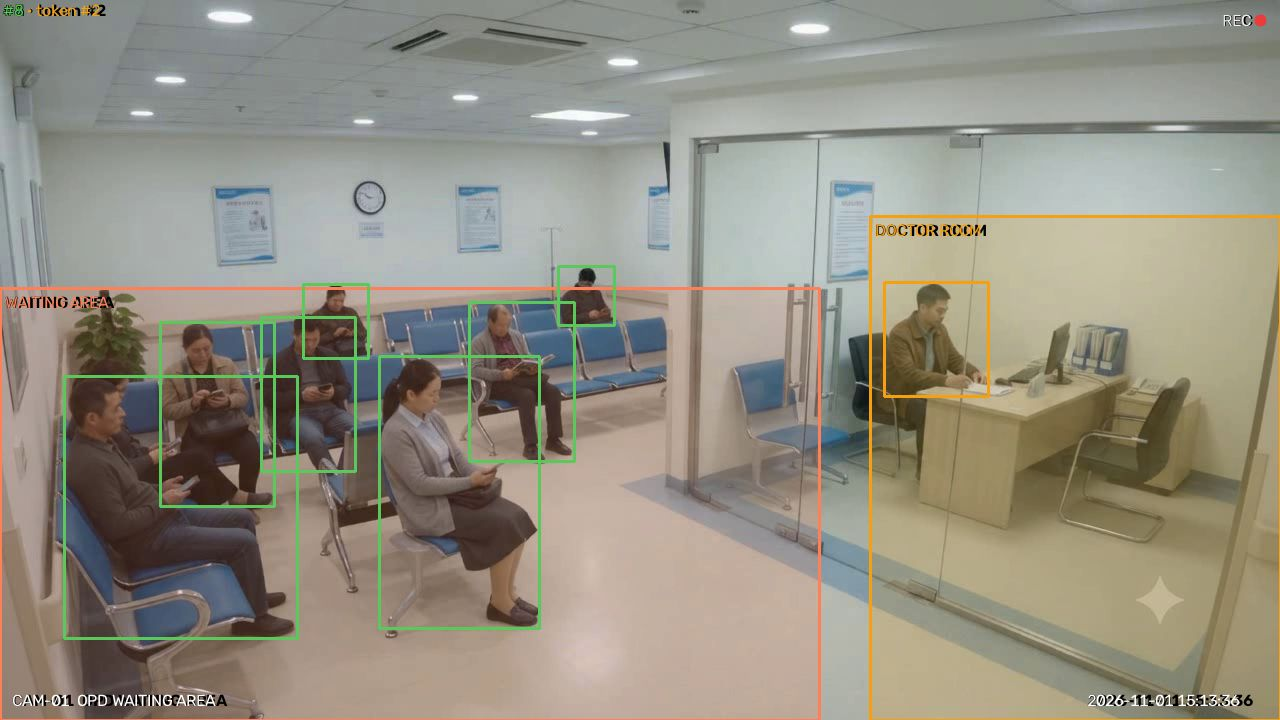
\includegraphics[width=\columnwidth]{annotated_frame.jpg}
\caption{Annotated frame. The waiting and doctor zones are tinted, every person
carries a track id and, inside the doctor zone, an occupant tag, which is
either a token number or \texttt{ghost}. The camera label, timestamp and
recording dot are drawn server-side.}
\label{fig:frame}
\end{figure}

\section{Queue Rules}
\label{sec:queue}

A token moves through waiting, called, in and done, with skipped and no-show
reachable from waiting or called and re-queueable afterwards. When an entry is
confirmed the engine links a token in a fixed order: a token the nurse has
already called; otherwise, if camera-advance is on (it is on by default), the
next waiting token by priority flag and registration order; otherwise the
occupant is recorded as unlinked. The nurse can always step in with manual
enter and free, skip, no-show, re-queue, and an undo that returns the most
recent completed token to the queue and removes the matching measurement.

Every transition is written to the log with a reason code and a source. The
codes are \textsc{entry\_confirmed}, \textsc{pass\_by}, \textsc{exit\_linked},
\textsc{exit\_ghost}, \textsc{seam\_hold} and \textsc{rebound}; the sources are
camera, nurse, manual and simulation. During the demo this proved more useful
than expected. When a token advanced on its own we could say which person
caused it, and when a nurse corrected something the log showed that too.

\section{Fuzzy Wait-Time Estimation}
\label{sec:fuzzy}

\subsection{Learned consultation length}
Let $t^{(1)},\dots,t^{(n)}$ be the raw durations of the last $W=12$
consultations in video seconds. A factor $\kappa$ converts them into clinic
minutes, and the result is blended with an 8-minute prior $P$,
\begin{equation}
\hat{m} = (1-w)\,P + w\,\operatorname{median}_{i\le W}\!\left(\frac{\kappa\,t^{(i)}}{60}\right),
\end{equation}
with blending weight $w=\min(1,n/4)$. Keeping raw seconds rather than pre-scaled
minutes was a deliberate change. The operator can move $\kappa$ between 10 and
120 during a demonstration, and every stored measurement, including ranges
already on screen, is re-scaled consistently.

\subsection{Membership functions}
Five inputs are fuzzified with triangular and trapezoidal sets
(Fig.~\ref{fig:sets}): the learned length (short, medium, long), the amount of
evidence behind it (low, medium, high confidence), the spread of past
measurements through the coefficient of variation (tight, moderate, wide), the
queue position (none, few, many) and the progress
$p=(t_{\mathrm{now}}-t_{\mathrm{in}})/\bar{t}$ of the live consultation (just
started, mid, likely ending).

\begin{figure*}[t]
\centering
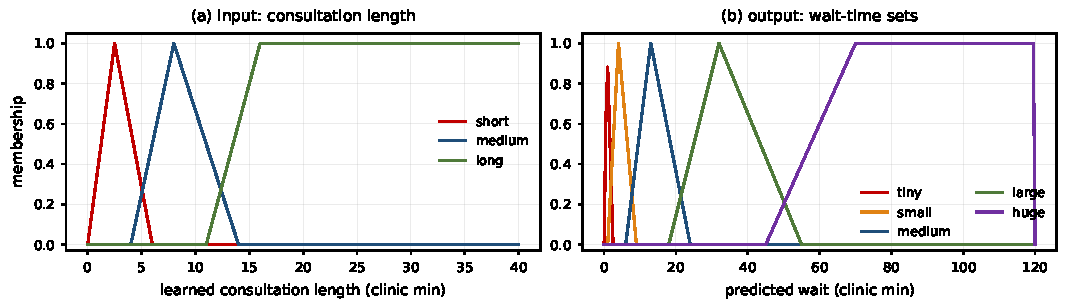
\includegraphics[width=\textwidth]{fig_fuzzy_sets.pdf}
\caption{Membership functions. (a) The learned consultation length is split into
short, medium and long sets. (b) The output is expressed over tiny, small,
medium, large and huge wait sets.}
\label{fig:sets}
\end{figure*}

\subsection{Rules and defuzzification}
Table~\ref{tab:rules} lists the rule base. Rule strength is the minimum of the
antecedents, rules are aggregated by maximum, and the result is defuzzified by
centroid over a discretized universe $X=\{0,0.5,\dots,120\}$ clinic minutes,
\begin{equation}
y^{*} = \frac{\sum_{x\in X} x\,\mu(x)}{\sum_{x\in X}\mu(x)},
\qquad
\mu(x)=\max_{r}\min\!\big(\alpha_r,\mu_{C_r}(x)\big).
\end{equation}
Bounds come from the same fuzzy state instead of a fixed percentage,
\begin{equation}
s = 0.18 + 0.32\,\mu_{\mathrm{wide}} + 0.22\,(1-\mu_{\mathrm{high}}),
\end{equation}
\begin{equation}
[y^{-},y^{+}] = \big[y^{*}(1-s),\ y^{*}(1+1.15\,s)\big].
\end{equation}
Sparse or erratic measurements therefore widen the interval rather than
pretending precision. If the current consultation has already overrun its
average, the ending rule fires and pulls the first waiting patient towards
``almost your turn''. Figure~\ref{fig:curve} shows the resulting surface: the
wait grows with queue position and with the learned length, and it grows fastest
for long consultations.

\begin{table}[t]
\caption{Rule base (antecedent $\rightarrow$ consequent)}
\label{tab:rules}
\centering
\small
\begin{tabular}{@{}ll@{}}
\toprule
Antecedent & Consequent \\
\midrule
length short $\wedge$ ahead none & wait tiny \\
length short $\wedge$ ahead few & wait small \\
length short $\wedge$ ahead many & wait medium \\
length medium $\wedge$ ahead none & wait small \\
length medium $\wedge$ ahead few & wait medium \\
length medium $\wedge$ ahead many & wait large \\
length long $\wedge$ ahead none & wait medium \\
length long $\wedge$ ahead few & wait large \\
length long $\wedge$ ahead many & wait huge \\
progress ending $\wedge$ ahead none & wait tiny \\
confidence low & wait medium (weight 0.6) \\
\bottomrule
\end{tabular}
\end{table}

\begin{figure}[t]
\centering
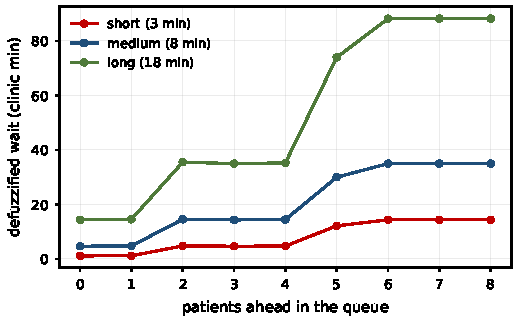
\includegraphics[width=0.92\columnwidth]{fig_fuzzy_curve.pdf}
\caption{Defuzzified wait against queue position for three learned lengths
(8 samples, moderate spread, consultation at 30\,\% of its expected length).}
\label{fig:curve}
\end{figure}

\subsection{What the patient sees}
Each waiting token is exposed as a range, a confidence tag and a phrase. The
nurse reads entries such as ``5--19 min, low confidence''; the patient display
shows ``about 5--18 min'' with the expected clock time and the number of people
ahead. Where the model is unsure the phrase becomes deliberately vague, and we
consider that a feature. A confident-looking number that turns out to be wrong
is worse for trust than an honest range.

\section{Interfaces}
\label{sec:ui}

All three pages poll \texttt{/api/state} once a second, so any screen can run on
any device on the local network.

The monitoring console (Fig.~\ref{fig:monitor}) shows the annotated feed, the
two crowd counters, the occupant list of the doctor room and the event log. It
also carries the zone editor. Zones are stored per clip, which matters during a
demo because switching sources keeps the framing of each clip separate. Auto
detection is deliberately conservative: it proposes a door only when the
cluster of disappearing people sits near a frame edge, and otherwise asks the
operator to draw it.

The nurse desk (Fig.~\ref{fig:nurse}) is the working surface. It has
registration with a priority flag, the live queue with a NEXT marker, call,
skip, no-show and re-queue, undo of the last consultation, CSV export, the
camera-advance toggle and the time-factor slider. Moving the slider re-scales
the estimates while the queue is running, which is how we match the pace of a
staged demonstration without restarting anything.

The patient display (Fig.~\ref{fig:patient}) is a kiosk board. It shows what is
being served, the next token (flashing ``please proceed'' when it is called),
how many people are waiting, and a per-token lookup giving the people ahead, the
range, the phrase, the expected clock time and the number of consultations the
estimate is based on.

\begin{figure}[t]
\centering
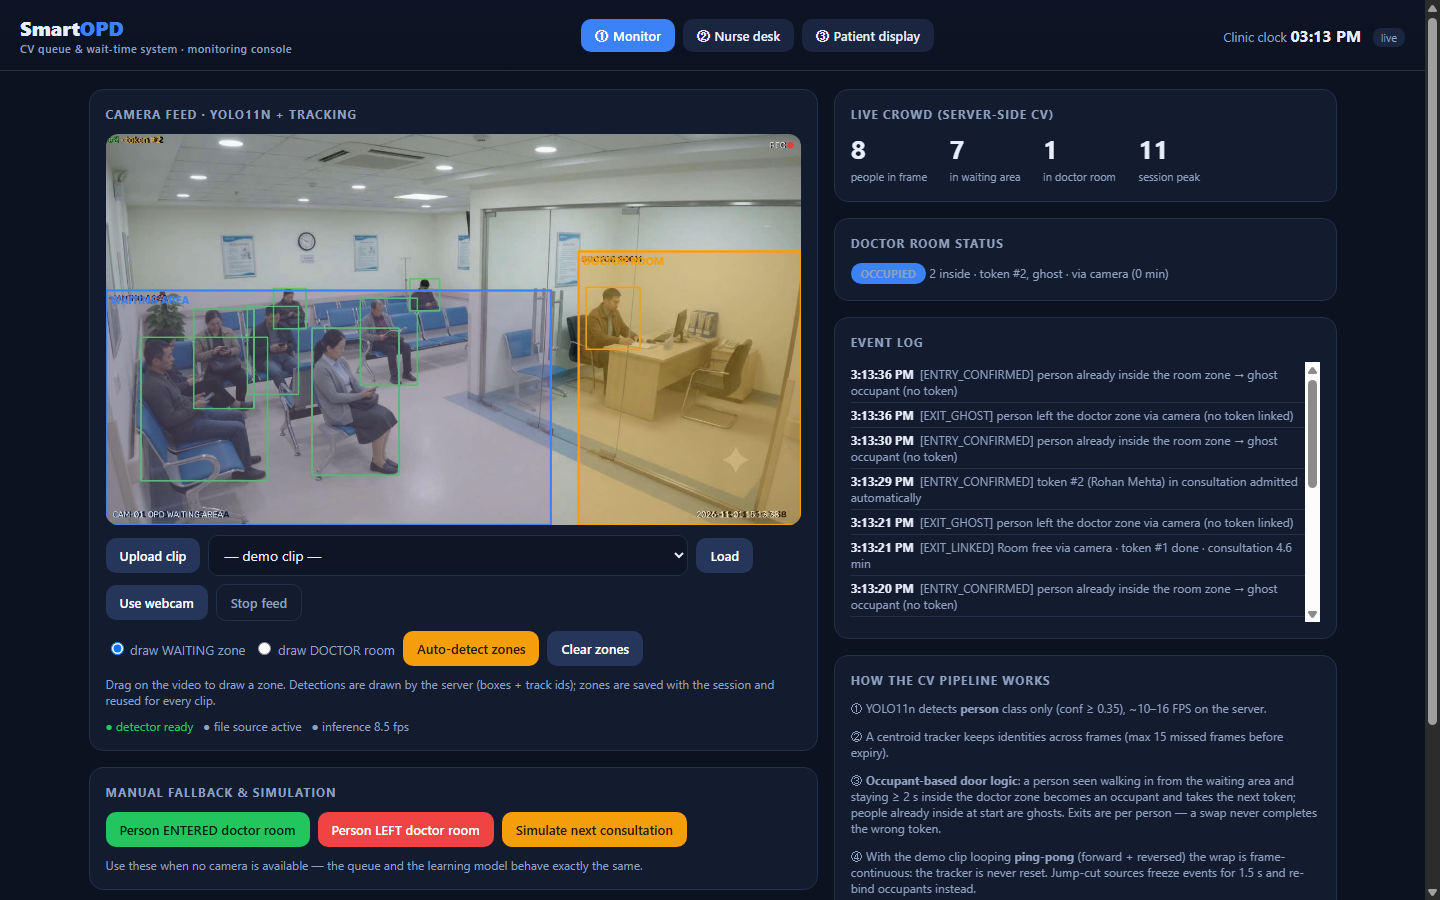
\includegraphics[width=0.88\columnwidth]{monitor.png}
\caption{Monitoring console with the annotated feed, crowd counters, room
occupants and the reason-coded event log.}
\label{fig:monitor}
\end{figure}

\begin{figure}[t]
\centering
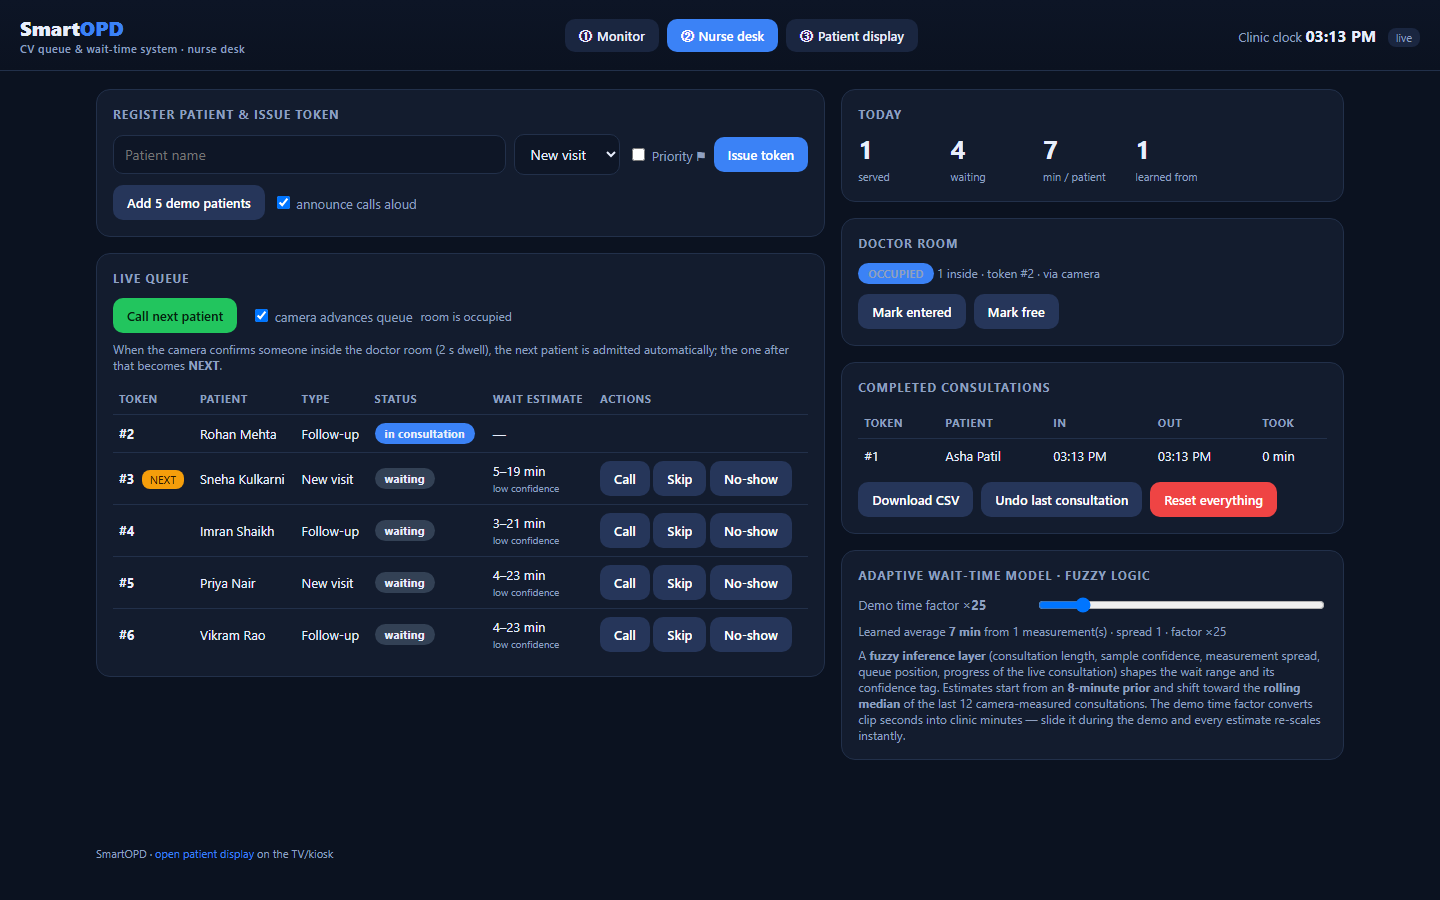
\includegraphics[width=0.88\columnwidth]{nurse.png}
\caption{Nurse desk with the NEXT marker, fuzzy ranges and confidence tags, the
occupant list, completed consultations with undo, and the time-factor slider.}
\label{fig:nurse}
\end{figure}

\begin{figure}[t]
\centering
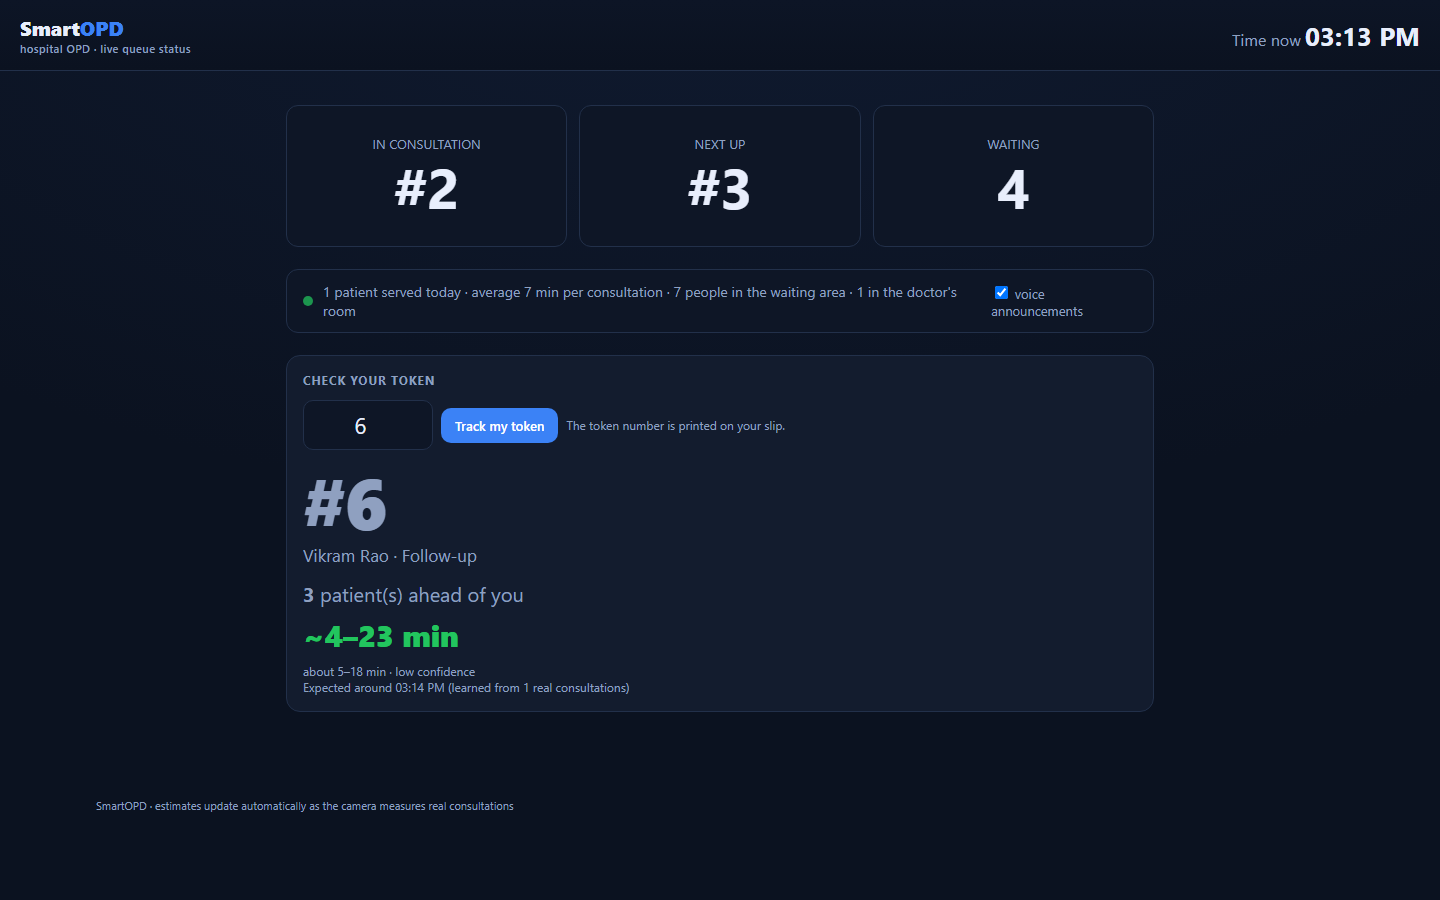
\includegraphics[width=0.88\columnwidth]{patient.png}
\caption{Patient display with the now-serving board and a per-token estimate
including a plain-language phrase.}
\label{fig:patient}
\end{figure}

\section{Evaluation}
\label{sec:eval}

\subsection{Unit tests}
The suite has 58 tests and runs in under a second on CPU
(Table~\ref{tab:tests}). Vision tests receive an injected clock, so time-based
rules are tested deterministically rather than by sleeping. A few properties
are tested as invariants: more people ahead never shortens a wait, and sparse
data never narrows the bounds. These two caught regressions while we tuned the
sets and cost almost nothing to keep.

\begin{table}[t]
\caption{Test suites and what they pin down}
\label{tab:tests}
\centering
\small
\begin{tabular}{@{}lcp{4.3cm}@{}}
\toprule
File & \# & Coverage \\
\midrule
\texttt{test\_queue.py} & 31 & token lifecycle, priority order, occupant
admission, swap safety, ghost exits, no-backwards invariant, undo,
serialisation and migration, CSV \\
\texttt{test\_vision.py} & 17 & tracker identity and expiry, entry dwell,
pass-by, flicker, vanish exits, seam hold and re-binding, continuous-loop
identity, crowd counting \\
\texttt{test\_fuzzy.py} & 10 & monotonicity in position and length, progress
sensitivity, confidence widening, prior fallback, label buckets \\
\bottomrule
\end{tabular}
\end{table}

\subsection{Headless replay}
The replay harness runs the real detector, tracker, analyzer and engine over the
ping-pong clip for three loops with six tokens waiting, using video time as the
engine clock. It checks that all six tokens complete, that they complete in
registration order, that no token ever leaves \texttt{in} for
\texttt{called} or \texttt{waiting}, and that every completed consultation trains
the estimator.

\begin{table}[t]
\caption{Replay results (six tokens, ping-pong clip, $\kappa=25$)}
\label{tab:replay}
\centering
\small
\begin{tabular}{@{}lcccc@{}}
\toprule
Token & Status & Raw $t$ (s) & Clinic (min) & Learned \\
\midrule
\#1 & done & 11.0 & 4.6 & yes \\
\#2 & done & 4.6  & 1.9 & yes \\
\#3 & done & 11.0 & 4.6 & yes \\
\#4 & done & 4.6  & 1.9 & yes \\
\#5 & done & 11.0 & 4.6 & yes \\
\#6 & done & 4.6  & 1.9 & yes \\
\midrule
\multicolumn{2}{@{}l}{completed / learned} & \multicolumn{3}{l}{6/6 \quad 6/6} \\
\bottomrule
\end{tabular}
\end{table}

The alternating durations come from the clip itself. The door is entered from
one side and left from the other, so the forward and reverse halves alternate
long and short stays. This is exactly the case that broke the earlier revert
rule; under the current semantics both durations are valid consultations and the
queue advances on each exit (Table~\ref{tab:replay}). The replay also shows the
intended invariants at work. The woman who is inside at $t=0$ is admitted as a
ghost and her exit is logged \textsc{exit\_ghost} without touching a token,
while the man who walks in consumes token \#1.

\subsection{Live operation}
With the demo clip running, the monitor reports 15 to 19 people in frame at 10 to
16 processed frames per second on CPU, with two occupants inside the doctor zone
during a swap. Immediately after a single measurement the estimator behaves as
expected for thin evidence: wide ranges such as 5--19, 3--21 and 4--23 minutes
for successive queue positions, all tagged low confidence. Moving the factor
from $\times25$ to $\times120$ re-scales the same measurements at once.

\subsection{What we did not measure}
We do not report precision and recall for door events, or mean absolute error
for the estimates. The project has no frame-level ground truth annotation, and
producing one from the same detector would be circular. A proper field study
needs a hand-labelled subset of entry and exit events ($F_1$ and latency) and a
log of realised consultation times (MAE and interval coverage). We list this as
the first item of future work instead of inventing numbers.

\section{Limitations}
\label{sec:limits}

The camera does not know who anybody is. The system assumes queue order: the
person who walks in is the next token. That is reasonable for a single-server
OPD, but a patient who jumps the queue will consume somebody else's token, and
the nurse has to correct it with undo. Verifying identity needs person
re-identification \cite{zheng2016reid}, which we have not attempted.

The design covers one doctor zone and one queue. More rooms would need
per-zone occupants and per-room queues; the data structures allow it but the
interface does not expose it yet.

The patient has to stay visible inside the zone while consulting. If the room
is out of view, the nurse falls back to manual enter and free, and the camera
becomes a crowd counter. Occlusion at the door can delay an exit by up to the
miss budget.

The factor $\kappa$ is a calibration, not a measurement. It is exposed, logged
and changeable at runtime precisely because no single value is correct for a
staged video.

On privacy, frames are processed in memory and never written to disk or sent
anywhere; only anonymous counters, token numbers, durations and zone rectangles
persist. A deployed system would still need signage, institutional approval and
probably face blurring at capture time.

\section{Conclusion and Future Work}
\label{sec:concl}

An inexpensive camera and a disciplined event model are enough to turn an OPD
waiting hall into a measurable queue. Entries and exits are attributed per
person, tokens advance without nurse input, and the wait estimate becomes a
range with an honest confidence tag rather than a single number that pretends to
be exact. The implementation is small, offline and auditable, and the rules that
mattered most are covered by tests.

Future work follows the limitations. We want a field study with annotated door
events and realised consultation times to report $F_1$ and ETA error honestly.
Person re-identification at the door would let the system verify the admitted
patient instead of trusting queue order. Multi-room and multi-camera operation
is a matter of duplicating the zone and queue structures and reworking the
nurse view. A patient-side QR check-in would give registration and queue state a
single identifier. Finally, integration with a hospital information system would
replace the CSV export, which is the current hand-off point.

\section*{Reproducibility}
The implementation, tests, replay harness and demo clips are released under the
MIT licence.\footnote{Source:
\url{https://github.com/Gauravguddeti/SmartOPD-CV-based-OPD-Queue-Wait-Time-System}}
The pipeline runs offline after a one-command setup that installs a local Python
environment and a 6\,MB detector weight file.

\begin{thebibliography}{16}

\bibitem{cayirli2003}
T.~Cayirli and E.~Veral, ``Outpatient scheduling in health care: A review of
literature,'' \emph{Production and Operations Management}, vol.~12, no.~4,
pp. 519--549, 2003.

\bibitem{gupta2008}
D.~Gupta and B.~Denton, ``Appointment scheduling in health care: Challenges and
opportunities,'' \emph{IIE Transactions}, vol.~40, no.~9, pp. 800--819, 2008.

\bibitem{redmon2016yolo}
J.~Redmon, S.~Divvala, R.~Girshick, and A.~Farhadi, ``You only look once:
Unified, real-time object detection,'' in \emph{Proc. IEEE Conf. Computer
Vision and Pattern Recognition (CVPR)}, 2016, pp. 779--788.

\bibitem{redmon2018yolov3}
J.~Redmon and A.~Farhadi, ``YOLOv3: An incremental improvement,''
\emph{arXiv preprint arXiv:1804.02767}, 2018.

\bibitem{ultralytics2024}
Ultralytics, ``YOLO11: Ultralytics YOLO documentation,'' 2024. [Online].
Available: \url{https://docs.ultralytics.com/models/yolo11/}

\bibitem{bewley2016sort}
A.~Bewley, Z.~Ge, L.~Ott, F.~Ramos, and B.~Upcroft, ``Simple online and
realtime tracking,'' in \emph{Proc. IEEE Int. Conf. Image Processing (ICIP)},
2016, pp. 3464--3468.

\bibitem{wojke2017deepsort}
N.~Wojke, A.~Bewley, and D.~Paulus, ``Simple online and realtime tracking with
a deep association metric,'' in \emph{Proc. IEEE Int. Conf. Image Processing
(ICIP)}, 2017, pp. 3645--3649.

\bibitem{zhang2022bytetrack}
Y.~Zhang \emph{et al.}, ``ByteTrack: Multi-object tracking by associating every
detection box,'' in \emph{Proc. European Conf. Computer Vision (ECCV)}, 2022,
pp. 1--21.

\bibitem{sindagi2018}
V.~A. Sindagi and V.~M. Patel, ``A survey of recent advances in CNN-based
single image crowd counting and density estimation,'' \emph{Pattern
Recognition Letters}, vol.~107, pp. 3--16, 2018.

\bibitem{gross2018}
D.~Gross, J.~F. Shortle, J.~M. Thompson, and C.~M. Harris, \emph{Fundamentals
of Queueing Theory}, 5th~ed. Hoboken, NJ, USA: Wiley, 2018.

\bibitem{zadeh1965fuzzy}
L.~A. Zadeh, ``Fuzzy sets,'' \emph{Information and Control}, vol.~8, no.~3,
pp. 338--353, 1965.

\bibitem{mamdani1975}
E.~H. Mamdani and S.~Assilian, ``An experiment in linguistic synthesis with a
fuzzy logic controller,'' \emph{International Journal of Man-Machine Studies},
vol.~7, no.~1, pp. 1--13, 1975.

\bibitem{ross2010fuzzy}
T.~J. Ross, \emph{Fuzzy Logic with Engineering Applications}, 3rd~ed.
Chichester, U.K.: Wiley, 2010.

\bibitem{zheng2016reid}
L.~Zheng, Y.~Yang, and A.~G. Hauptmann, ``Person re-identification: Past,
present and future,'' \emph{arXiv preprint arXiv:1610.02984}, 2016.

\bibitem{fastapi2024}
S.~Ram\'irez, ``FastAPI documentation,'' 2024. [Online]. Available:
\url{https://fastapi.tiangolo.com}

\end{thebibliography}

\end{document}
